%Redigé par Théo Falgarone et Tristan Maunier 

\documentclass[a4paper, 12pt]{report}
%
\usepackage[english,french]{babel} %Import french package for every keyword like Table of contents -> Table des matieres
\usepackage{float}
\usepackage[utf8]{inputenc}
\usepackage[Ot1,T1]{fontenc}
\usepackage[top=2.5cm, bottom=3cm, left=2.5cm, right=2.5cm]{geometry}
\usepackage{graphicx}
\usepackage{colortbl}

\setcounter{tocdepth}{3} %Limits depth in the table of content of sections showed
\setcounter{secnumdepth}{4} %Limits numerotation, in order to avoid Section 1.1.1.1.1...

\usepackage{listings} %Package that allow us to put code in the report

\begin{document}
	\begin{titlepage}
    	\begin{center}
		\vfill
		\Huge{OSS 117 : Eye Origin\\
        Cahier des charges}
		\vfill
		\end{center}
		\begin{center}
	        \centering
\includegraphics[height=3cm]{univ.jpg}\hfill \\
	    
		\LARGE{Université de Bordeaux}\\
		 Théo Falgarone et Tristan Maunier \\
		\vfill
		\vfill
         \end{center}
                 \begin{minipage}{0.4\textwidth}
\begin{center} \large
\emph{Clients:} \\
Adrien \textsc{Boussicault} % Supervisor's Name
\par Pierre \textsc{Lacroix} % Supervisor's Name
\end{center}
\end{minipage}\\[2cm]
	\end{titlepage}
	
    %Create the table of contents
    \tableofcontents
    
    %We have to reset the counter because Introduction is always the page number 1
    \setcounter{page}{0} 
    	
	\chapter*{Contexte} %The star protects the chapter to be counted
		\addcontentsline{toc}{chapter}{Contexte} 
		Le présent document explique comment, à partir d'un flux d'images contenant les yeux et l'iris de l'utilisateur on peut positionner le curseur de la souris à l'endroit sur l'écran où l'utilisateur regarde.
	\chapter{Fonctionnement général du logiciel}
    \section*{Flux de tâches général}
    La figure 1.1 représente l'ensemble des tâches successives que doit remplir le logiciel ainsi que les différents éléments concernés par ces tâches. En bleu les entrées et les sorties des actions représentées en rouge et en vert les algorithmes entrant en jeu lors de la réalisation de ces actions. Au fur et à mesure de la succession de ces tâches différents besoins fonctionnels liés au logiciel vont être identifiés. Ce flux de tâches ainsi que les besoins fonctionnels déterminées seront détaillés dans les parties suivantes du document.
    \begin{figure}[!h]
    \centering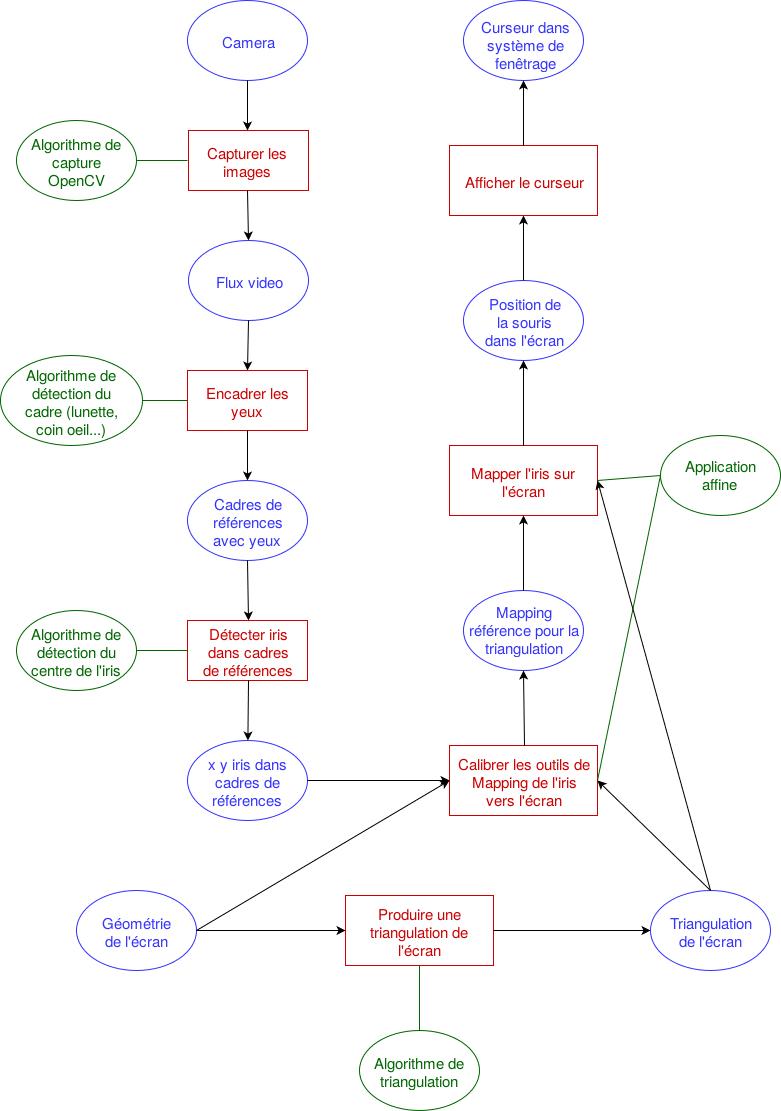
\includegraphics[height=22cm]{workflow.png}
    \caption{Flux de tâches du logiciel}
    \end{figure}
    \section{Capturer les images}
		La capture d'images est effectuée à partir d'un flux vidéo obtenu grâce à une caméra positionnée devant l'utilisateur. Un système physique permet d'orienter la caméra selon des angles d'inclinaison et de rotation précis, de plus la caméra peut être disposée à une hauteur souhaitée tout autour de l'écran. La bibliothèque de traitement d’images OpenCV\cite{c1} permet de traiter le flux vidéo et d'en ressortir les images d'intérêt. Chaque image capturée doit contenir le visage et donc les yeux de l'utilisateur. Plusieurs contraintes sont liées à la capture des images, notamment la luminosité de la pièce qui peut altérer la détection de l'oeil. La résolution de la caméra joue un rôle important dans la qualité de l'analyse de ces images, en effet si la résolution n'est pas suffisamment élevée les images capturées ne pourront pas être utilisées par le logiciel. La présence d'une ou plusieurs caméras est également un facteur à déterminer.  
\newpage 
	\section{Suivre les yeux}
        Du fait des mouvements de l'utilisateur, il est difficile de positionner avec précision le centre de son iris dans l'image sans référencement. On doit pouvoir détecter les yeux de l'utilisateur dans l'image et en déduire une coordonnée correspondant au centre de l'iris pour chacun des deux yeux. C'est pourquoi un repère est défini dans l'image afin de suivre l'oeil et ainsi produire une image indépendante contenant l'oeil dans sa totalité. Ce repère servira de nouveau repère vis à vis duquel sera positionné le centre de l'iris de l'oeil. Nous avons identifié deux solutions techniques pouvant répondre à ce besoin.
        \subsection{Définir un cadre à détecter autour de l'oeil}
L'utilisateur porte des lunettes rectangles pouvant être repérées par un algorithme de détection, les lunettes doivent être suffisamment larges pour encadrer la totalité de l'oeil. En pratique le cadre rectangle des lunettes ne sera pas rectangle dans l'image, on parlera ici d'un quadrilatère du fait des angles d'orientation de la caméra et/ou de la position de l'utilisateur. Une image bornée par ce cadre, dit "de référence",est extraite de l'image initiale et subira une transformation afin que l'image soit contenue dans un véritable rectangle. Ce rectangle servira de nouveau repère afin de positionner l'iris.
\subsubsection{Stocker les coordonnées du cadre de référence}
La position du cadre de référence dans l'image initiale doit être sauvegardée, les coordonnées pour chaque cadre et chaque image seront stockées dans un fichier texte.
		\subsection{Détecter le coin de l'oeil}
Définir le coin de l'oeil comme repère dans l'image est une alternative au port des lunettes. En effet le coin de l'oeil peut servir d'origine pour un nouveau repère dans lequel se trouvera, à l'instar du cadre des lunettes, l'iris de l'utilisateur.
\subsubsection{Stocker les coordonnées du coin de l'oeil}
La position du coin de l'oeil dans l'image est stockée pour chaque image dans un fichier texte. 

    \section{Calculer la coordonnée du centre de l'iris dans un nouveau repère}
    Une fois le nouveau repère défini pour chaque oeil, un algorithme doit détecter le centre de l'iris et en ressortir la position de ce dernier sous forme de coordonnées en abscisse et en ordonnée (x et y).
\subsection{Stocker les coordonnées de l'iris}
Ces coordonnées sont enregistrées dans un fichier texte organisé par oeil et par image capturée.
    	\section{Obtenir la géométrie de l'écran}
	Les écrans présentent des dimensions différentes, la taille de l'écran de l'utilisateur doit donc être récupérée dans un premier lieu afin de pouvoir effectuer correctement les étapes de mapping et de triangulation.
	\section{Produire une triangulation de l'écran}
	Pour positionner le curseur à l'écran via une position de l'iris donnée, il est indispensable de se rapporter à un même référentiel. La triangulation est une méthode permettant de découper un plan en une multitude de triangles, dans notre cas le plan à trianguler est l'écran. Une triangulation possible de l'écran avec 9 points pourrait être la suivante :
	\begin{figure}[!h]
		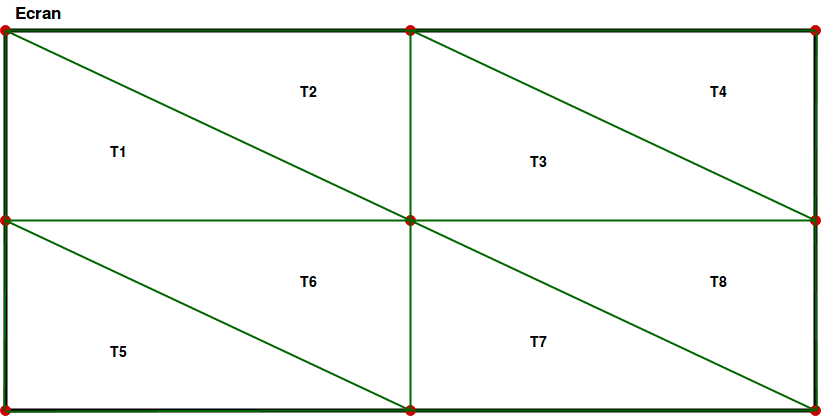
\includegraphics[scale=0.6]{triangulation_ecran.png}
		\caption{Exemple de triangulation de l'écran avec 9 points}	
	\end{figure}
	\newpage	  
	\section{Calibrer la détection de l'iris}
	Afin de pouvoir transposer un point correspondant à la position de l'iris vers un triangle tracé à l'écran, il faut appliquer la même méthode pour trianguler la zone dans laquelle peut se déplacer l'iris lorsque l'utilisateur regarde l'écran. Pour ce faire on peut imaginer une étape de calibration, où l'utilisateur doit successivement fixer neuf points à l'écran. A chaque point, les coordonnées issues de l'algorithme de détection de l'iris sont enregistrées et permettent de dessiner une triangulation de la même manière que pour la triangulation de l'écran.
	\begin{figure}[!h]
		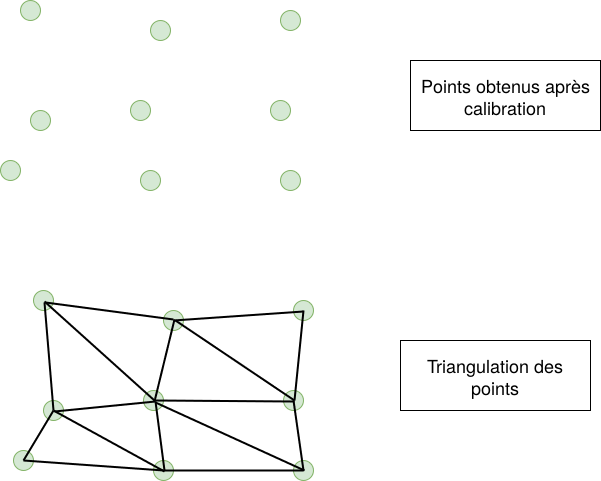
\includegraphics[scale=0.8]{calibration.png}
		\caption{Exemple de triangulation après calibration}	
	\end{figure}
	\newpage	
	\section{Identifier le triangle contenant le point}
	Afin de pouvoir prétendre transformer la position du centre de l'iris contenu dans l'un des triangles tracés lors de l'étape de calibration en point sur l'écran, on doit détecté le dit triangle contenant ce point ainsi que son homologue localisé sur l'écran. En effet chaque triangle tracé que ce soit lors de la calibration ou lors de l'étape de mappage de l'écran est une entité géométrique unique indépendante des autres triangles, cependant un triangle issu de la calibration correspond à un triangle spécifique à l'écran. Si on se réfère aux figures 1.2 et 1.3, on remarque par exemple que le triangle T1' est l'homologue du triangle T1 et inversement.
	
	\section{Transposer la position d'un point dans un triangle vers un second triangle}
	Une fois le triangle contenant le centre de l'iris détecté identifié, il s'agit donc de transposer ce point vers l'écran. Pour transposer un point d'un repère vers un second, ici nos repères sont des triangles, il nous faut effectuer une application affine sur ce point\cite{c2}. Prenons exemple avec les triangles T1 et T1' vu en figure 1.2 et 1.3, l'application affine envoie le point P' sur T1, donnant ainsi le point P. (voir figure 1.4). L'application affine sur le point P s'écrit de la manière suivante : \\
	$$
	\overrightarrow{f}(P') = \overrightarrow{\varphi _{2}} (\overrightarrow{\varphi _{1}^{-1}}(P'))\\
	$$
		\\
$\varphi _{2}$ et $\varphi _{1}^{-1}$ sont des applications linéaires permettant de transformer les repères des triangles vers un même repère i,j orthonormé, elles doivent être calculées afin de pouvoir résoudre l'équation de l'application affine.
		\subsection{Application linéaire}
		L'application linéaire est une application sur deux espaces vectoriels qui respectent l'addition des vecteurs et les produits scalaires définis dans ces espaces vectorielles. Soit E et F deux espaces vectorielles sur un corps K, une application $ f : E \longrightarrow F $ est dite linéaire si elle vérifie à la fois : \\
		$$
		\forall x,y \in E  f(x+y) = f(x) + f(y)\\
		\vspace{0.2cm}
		\\
		\forall \lambda \in K  \forall x,y  \in E  f(\lambda x) = \lambda f(x)\\
		$$
		\\
		L'application f est linéaire si et seulement si :\\
		$$
		\forall x,y \in E \forall \lambda , \mu \in K  f(\lambda x + \mu y) = \lambda f(x) + \mu f(y)\\
		$$
		\\
		En reprenant l'exemple en figure 1.4 l'application linéaire de $\varphi_{1}$ se détermine de la manière suivante : \\
		Ici, a, b, c et d sont les coefficients du triangle T1' que l'on transpose dans le repère $\overrightarrow{i},\overrightarrow{j}$.
		$$
		\left(\begin{array}{cc}
		a & b \\
		c & d 
		\end{array}
		\right) _{\overrightarrow{i}\overrightarrow{j} \rightarrow \overrightarrow{i}\overrightarrow{j}}
		\left(\begin{array}{c}
		1 \\
		0 
		\end{array}
		\right) _{\overrightarrow{i}\overrightarrow{j}} 
		\longrightarrow
		\left(\begin{array}{c}
		a\\
		c
		\end{array}
		\right)
		$$
		$$
		\left(\begin{array}{cc}
		a & b \\
		c & d 
		\end{array}
		\right) _{\overrightarrow{i}\overrightarrow{j} \rightarrow \overrightarrow{i}\overrightarrow{j}}
		\left(\begin{array}{c}
		0 \\
		1 
		\end{array}
		\right) _{\overrightarrow{i}\overrightarrow{j}} 
		\longrightarrow
		\left(\begin{array}{c}
		b\\
		d
		\end{array}
		\right)
		\\
		$$
		
		On en déduit $\varphi _{1} (\overrightarrow{i})$ et $\varphi _{1} (\overrightarrow{j})$ :
		$$
		\varphi _{1} (\overrightarrow{i}) = C' - A' = \left(\begin{array}{c}
		C' _{i} - A' _{i} \\
		C' _{j} - A' _{j}
		\end{array}
		\right)
		\\
		$$
		$$
		\varphi _{1} (\overrightarrow{j}) = B' - A' = \left(\begin{array}{c}
		B' _{i} - A' _{i} \\
		B' _{j} - A' _{j}
		\end{array}
		\right)
		\\
		$$
		
		On peut donc écrire :
		$$
		\left(\begin{array}{cc}
		C' _{i} - A' _{i} & B' _{i} - A' _{i} \\
		C' _{j} - A' _{j} & B' _{j} - A' _{j} 
		\end{array}
		\right) _{\overrightarrow{i}\overrightarrow{j} \rightarrow \overrightarrow{i}\overrightarrow{j}} = {\cal \overrightarrow{\varphi _{1}}}
		$$
		\\
		
		L'application linéaire de $\varphi_{2}$ se détermine de la manière suivante : \\
		Ici, a, b, c et d sont les coefficients du triangle T1 que l'on transpose dans le repère $\overrightarrow{i},\overrightarrow{j}$.
		$$
		\left(\begin{array}{cc}
		a & b \\
		c & d 
		\end{array}
		\right) _{\overrightarrow{i}\overrightarrow{j} \rightarrow \overrightarrow{i}\overrightarrow{j}}
		\left(\begin{array}{c}
		1 \\
		0 
		\end{array}
		\right) _{\overrightarrow{i}\overrightarrow{j}} 
		\longrightarrow
		\left(\begin{array}{c}
		a\\
		c
		\end{array}
		\right)
		$$
		$$
		\left(\begin{array}{cc}
		a & b \\
		c & d 
		\end{array}
		\right) _{\overrightarrow{i}\overrightarrow{j} \rightarrow \overrightarrow{i}\overrightarrow{j}}
		\left(\begin{array}{c}
		0 \\
		1 
		\end{array}
		\right) _{\overrightarrow{i}\overrightarrow{j}} 
		\longrightarrow
		\left(\begin{array}{c}
		b\\
		d
		\end{array}
		\right)
		\\
		$$
		
		On en déduit $\varphi _{2} (\overrightarrow{i})$ et $\varphi _{2} (\overrightarrow{j})$ :
		$$
		\varphi _{2} (\overrightarrow{i}) = C - A = \left(\begin{array}{c}
		C _{i} - A _{i} \\
		C _{j} - A _{j}
		\end{array}
		\right)
		\\
		$$
		$$
		\varphi _{2} (\overrightarrow{j}) = B - A = \left(\begin{array}{c}
		B _{i} - A _{i} \\
		B _{j} - A _{j}
		\end{array}
		\right)
		\\
		$$
		
		On peut donc écrire :
		$$
		\left(\begin{array}{cc}
		C _{i} - A _{i} & B _{i} - A _{i} \\
		C _{j} - A _{j} & B _{j} - A _{j} 
		\end{array}
		\right) _{\overrightarrow{i}\overrightarrow{j} \rightarrow \overrightarrow{i}\overrightarrow{j}} = {\cal \overrightarrow{\varphi _{2}}}
		$$
		\\
		
		De $\varphi_{1}$ nous pouvons en déduire $\varphi _{1}^{-1}$ :
		\\
		$$
		\left(\begin{array}{cc}
		C _{i} - A _{i} & B _{i} - A _{i} \\
		C _{j} - A _{j} & B _{j} - A _{j} 
		\end{array}
		\right) _{\overrightarrow{i}\overrightarrow{j} \rightarrow \overrightarrow{i}\overrightarrow{j}} ^{-1} = {\cal \overrightarrow{\varphi _{1}^{-1}}}
		\\
		$$
		$$
		\frac{1}{det(\varphi _{1})}\times \left(\begin{array}{cc}
		B _{j} - A _{j} & -B _{i} + A _{i} \\
		-C _{j} + A _{j} & C _{i} - A _{i}  
		\end{array}
		\right) _{\overrightarrow{i}\overrightarrow{j} \rightarrow \overrightarrow{i}\overrightarrow{j}} = {\cal \overrightarrow{\varphi _{1}^{-1}}}
		\\
		$$

			\subsection{Application affine}
			Grâce aux deux applications linéaires réalisées auparavant, il est donc possible de réaliser l'application affine permettant de transposer la position de notre point d'intérêt vers l'écran.
			L'application affine du point P doit prendre en compte l'origine du repère, ici le point A, on obtient donc l'application affine suivante :\\
$$
f(P') = A + \overrightarrow{f}(P'-A) \\
$$
$$
f(P') = \left(\begin{array}{c} A _{i} \\ A _{j} \end{array}\right) + \overrightarrow{\varphi _{2}} \times \overrightarrow{\varphi _{1}^{-1}} \times \left(\begin{array}{c} P' _{i} - A _{i} \\ P' _{j} - A _{j} \end{array}\right)
\\
$$
$$
f(P') = A + \varphi _{2} \times \varphi _{1}^{-1} \times (P'-A) \\
\vspace{0.2cm}
\\
$$
\\ L'application  affine $f(P')$ calculée du point P' donne la position du point P contenu dans le triangle T1 à l'écran homologue du triangle T1' contenant le point P' initialement. 
\begin{figure}[!h]
	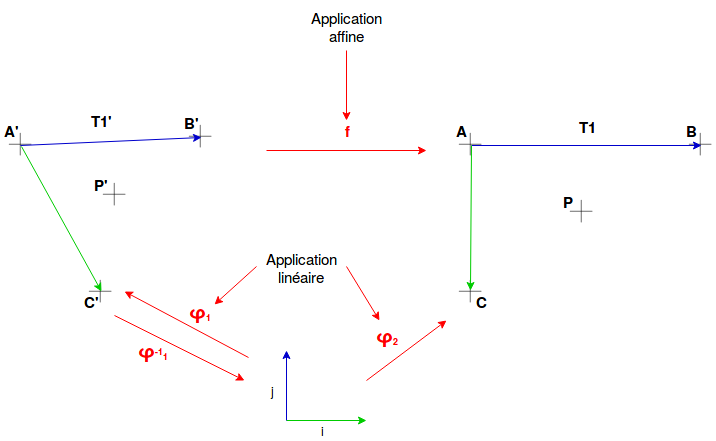
\includegraphics[scale=0.7]{application_affine.png}
	\caption{Transformation du point P' en P par l'application affine}
	\end{figure}

\newpage

    \section{Afficher le curseur}
		\subsection{Principe et définitions}
Une fois le logiciel capable de traduire une position de l'iris en position du curseur à l'écran, on se posent les questions de comment afficher ce curseur à l'écran et dans quels cas il doit s'afficher. \\
Plusieurs notions entrent en jeu lors de ce questionnement.\\
Lors d'un affichage informatique il est nécessaire de synchroniser l'affichage avec la fréquence de rafraîchissement de l'écran pour éviter des artefacts visuels déplaisants.
On parle de fréquence de rafraîchissement ( ou taux de rafraîchissement) de l'écran pour définir le nombre d'images maximal que l'écran peut afficher en une seconde, elle est exprimée en Hertz. On distingue ici le taux de  rafraîchissement de l'écran au nombre d'images que le dispositif vidéo utilisé est capable de fournir, ce nombre étant lui exprimé en fps(frame per second) ou images par seconde en français.
La fréquence de rafraîchissement d'un écran se situe entre 50 et 144 Hz, et les cadences usuellement employées par des dispositifs vidéos sont de 30,60 ou 100 fps. Pour information on peut traduire 1Hz par 1fps, la fréquence de rafraîchissement d'un écran se situe donc entre 50 et 144 fps.\\
L'enjeu ici est à la fois d'identifier l'endroit où l'oeil de l'utilisateur pointe sur l'écran mais aussi de déterminer quand l'information doit être captée afin de la traduire en position du curseur.\\
En se basant sur la publication "Modélisation cognitive computationnelle de la recherche d'information" \cite{c4}, On considère qu'au cours du temps, l'oeil peut se trouver dans deux configurations différentes:
\begin{itemize}
\item Soit l'oeil est dit "en mouvement" c'est à dire que la position de l'iris varie entre deux instants. Cette phase se décompose en deux étapes successives :
\begin{itemize}
\item Une phase de latence qui peut se traduire par la prise de temps de l'oeil de planifier le mouvement, qui dure entre 175 et 200 ms.
\item Une phase d'exécution du mouvement qui s'effectue une fois que cette phase de mouvement a été initiée, elle correspond au temps nécessaire pour déplacer réellement les yeux vers la cible. Ce temps d'exécution dépend de la distance entre la position initiale de l'oeil et la cible. Un mouvement de 2 degrès dure environ 30ms tandis qu'un mouvement de 5 degrès dure environ 40-50ms.
\end{itemize}
\item Soit l'oeil est dit en phase de "fixation" qui correspond à une période de temps où l'oeil est pratiquement maintenu vers une unique direction. Cette fixation dure entre 100 et 250ms. 
\end{itemize}
 
		\subsection{Quand relever la position de l'iris ?}
D'après la publication étudiée, la prise d'information sur la position de l'oeil est acquise uniquement lors de la phase de fixation de l'oeil. En effet ils ignorent la phase de mouvement qu'ils considèrent trop rapide, la vision y étant supprimée. Il s'agit donc d'identifier chaque phase de fixation et de récupérer une position de l'iris pour chacune d'elles.\\
Comme dit précédemment dans un soucis de confort visuel, le taux de rafraîchissement de l'écran doit être synchronisé avec la cadence vidéo. Le nombre de positions du curseur envoyées sur l'écran doit être alors limité par l'un ou l'autre des paramètres cumulé au nombre de phases de fixation identifiées.\\
Le but est de déterminer en fonction du taux de rafraîchissement de l'écran utilisé et de la cadence de la caméra utilisée le nombre d'images successives que le programme doit comparer afin de déterminer ou non s'il s'agit d'une phase de fixation de l'oeil. En effet grâce à la limite déterminée on obtient la fréquence d'images en ms qui correspond à une seconde divisée par la limite (pour une limite de 30 fps, on obtient une fréquence d'une image toutes les 33ms). Ensuite en divisant 250ms (durée d'une phase de fixation) par cette fréquence on obtient le nombre d'images à comparer. \\
On note Lim la limite définie en fps et Fq la fréquence d'images en ms. \\
$$ Fq = \frac{1}{Lim} $$ \\
et avec Nbi le nombre final d'images à comparées et df la durée de la phase de fixation fixée à 250ms on a \\
$$ Nbi = \frac{df}{Fq} $$ \\
On considère que si les coordonnées de l'iris détecté sont identiques sur toutes les images comparées alors il existe une phase de fixation et ainsi la position de l'iris est récupérée puis transformée en position du curseur. Dans le cas où les coordonnées varient une nouvelle phase de fixation est testée, c'est à dire qu'un nouveau lot d'images est comparé.\\
On considère ici qu'une phase de fixation dure toujours 250ms, ainsi si dans une seconde toutes les phases de fixations sont validées le logiciel renverra 4 positions successives du curseur à l'écran au cours de cette seconde. \\
Dans le tableau 1.1 ci-dessous sont regroupées des exemples de calculs du nombre d'images à comparer pour un taux de rafraîchissement de 50 ou 144 Hz et pour des cadences vidéo de 30, 60 et 100 images par secondes. 
\begin{center}
\begin{table}[!h]
\caption{Nombre d'images à comparer en fonction de la cadence vidéo et du taux de rafraîchissement de l'écran}
\vspace{0.5cm}
\begin{tabular}{|c|c|c|c|c|c|c|}
\hline
Cadence (fps) & \multicolumn{2}{c|}{30} & \multicolumn{2}{c|}{60} & \multicolumn{2}{c|}{100}\\
\hline
Taux de rafraîchissement (fps / Hz) & 50 & 144 & 50 & 144 & 50 & 144 \\
\hline
Limite (fps) & \cellcolor[RGB]{178,255,102} 30 & \cellcolor[RGB]{178,255,102} 30 & \cellcolor[RGB]{255,178,102} 50 & \cellcolor[RGB]{178,255,102} 60 & \cellcolor[RGB]{255,178,102} 50 & \cellcolor[RGB]{178,255,102} 100 \\
\hline
Fréquence d'images (ms) & 33 & 33 & 20 & 17 & 20 & 10 \\
\hline 
Nombre d'images comparées & 7 & 7 & 12 & 14 & 12 & 25 \\
\hline
\end{tabular}
\\
\end{table}
\end{center}
\begin{table}[!h]
\begin{tabular}{|c|c|}
\hline
\cellcolor[RGB]{178,255,102}{  } & Limité par la Cadence \\
\hline
\cellcolor[RGB]{255,178,102}{  } & Limité par le Taux de rafraîchissement de l'écran \\
\hline
\end{tabular}
\end{table}
    
    
    
    \chapter{Validation du modèle}
    	Le logiciel tel qu'il est imaginé fait appel à différents algorithmes, notamment de traitement d'images et de transformation de coordonnées. Certains algorithmes sont susceptibles de générer des erreurs ou de ne pas être suffisamment précis pour répondre aux besoins du logiciel. Nous avons identifié les principales erreurs pouvant être générées dans la figure 1.1. $e_{ref}$ est l'erreur générée par l'algorithme de détection du cadre. $e_{iris}$ est l'erreur générée par l'algorithme de détection du centre de l'iris. L'étape de calibration reprenant ces deux derniers algorithmes elle équivaut à $(e_{ref} + e_{iris})$. Cette étape de calibration étant répété plusieurs fois pour améliorer la précision du positionnement des points, nous considérons pour la suite de notre modèle que cette erreur est négligable et donc proche de 0. L'erreur issue de la transformation des coordonnées du centre de l'iris en coordonnées de curseur à l'écran est nommée $e_{aff}$. Enfin, $e_{fix}$ désigne l'erreur générée par le positionnement du curseur. $e_{max}$ représente l'erreur limite que l'ensemble des erreurs ne devra pas dépasser pour que l'utilisation du logiciel soit correct. Nous pouvons écrire la relation suivant :
    	$$
    	e_{max} \le e_{ref} + e_{iris} + (e_{ref} + e_{iris}) + e_{aff} + e_{fix}
    	$$
    	$$
    	e_{max} \le e_{ref} + e_{iris} + 0 + e_{aff} + e_{fix}
    	$$
    	\\
    	Afin de confirmer le bon fonctionnement des algorithmes clés, nous allons établir une succession de tests. Ces tests permettront d'évaluer individuellement des  algorithmes pouvant répondre à des besoins du logiciel et déterminer s'ils peuvent y être intégré.
    	\begin{figure}
    	\centering
    	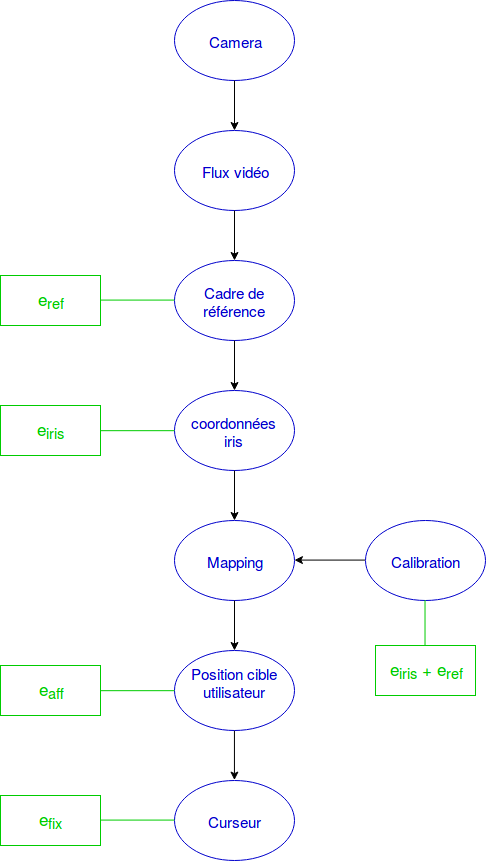
\includegraphics[scale=0.7]{flux_erreur.png}
    	\caption{Erreurs générées lors du flux de tâche du logiciel}
    	\end{figure}
    	\newpage
    	
    	\section{Déterminer l'erreur maximale tolérée pour l'utilisation du logiciel}
        	Comme décrit dans le chapitre 1, le logiciel a pour objectif de positionner avec précision le curseur sur l'écran via une reconnaissance de l'iris de l'utilisateur. La première étape de cette série de test est donc de déterminer avec quelle précision le curseur peut être positionné à l'écran sans provoquer de gêne pour l'utilisateur.\\
Pour ce faire, un test basé sur l'appréciation visuel de l'utilisateur est mis en place. En effet le but de cette opération est de tester à tour de rôle des erreurs de positionnement du curseur, il s'agira pour l'utilisateur de définir un nombre de pixels limite, que l'on appelera l'erreur $e_{max}$ , au delà duquel la sensation de "sursaut du curseur" est trop gênant lors d'une utilisation classique d'un ordinateur.\\
Dans un premier temps l'erreur en pixel est définie. Un cercle de rayon égal à cette erreur est tracée à l'écran, ce cercle regroupe l'ensemble des pixels où pourrait se trouver le curseur à un instant t selon l'erreur déterminée. On imagine une grille d'abscisse x et d'ordonnée y regroupant toutes les coordonnées possibles du curseur correspondant chacune à un pixel précis. Un écart fixe entre chaque instant t doit être défini (0,02 secondes par exemple) et à chaque instant t au cours du test le curseur prendra une position (x,y) aléatoire à l'intérieur de ce cercle.\\
En parallèle de cet événement, on déplacera ce cercle sur l'écran tout au long du test selon un parcours pré-défini afin de simuler un déplacement ordinaire de la souris sur un écran. Le cercle changera de position à tous les instants t' écartés les uns des autres d'un écart fixe (0.04 secondes par exemple). Un récapitulatif de l'opération de détermination de $e_{max}$ est présenté ci-dessous (Figure 2.1).
    \begin{figure}
    \centering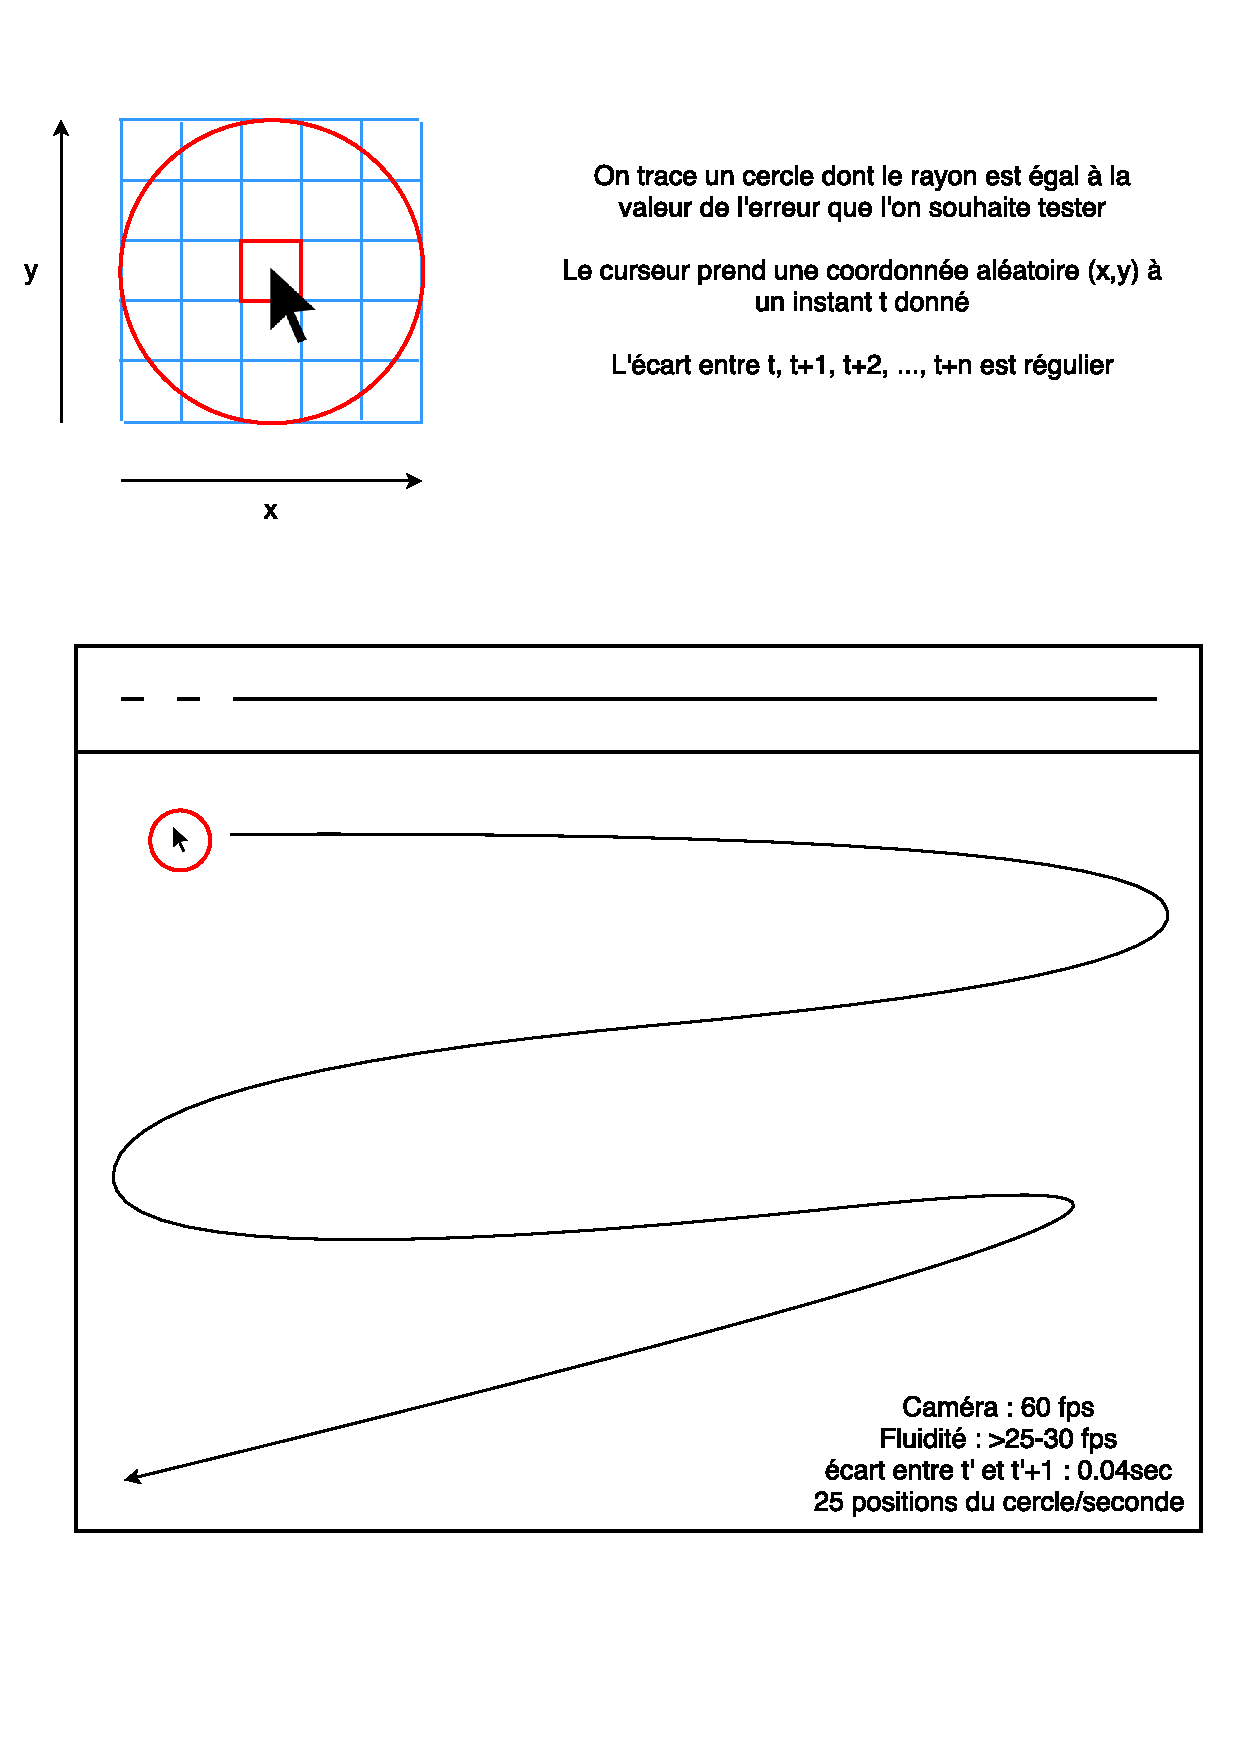
\includegraphics[height=24cm]{erreur_max.pdf}
    \caption{Schéma de la détermination de $e_{max}$ }
    \end{figure}
    \newpage
         
	\section{Transposition d'un point d'un triangle vers un autre par application affine}
		\subsection{Test de l'application affine}
         Afin de prouver que la transposition d'un point localisé dans un triangle vers un autre triangle via le calcul de l'application affine de ce point est fiable, il est nécessaire de tester cette opération au préalable sur des échantillons. 
On prédétermine un triangle construit à partir de trois points de coordonnées connues, on applique l'algorithme de l'application affine à un lot de points aléatoires également de coordonnées connues contenus dans ce triangle. On réalise ensuite le calcul manuel de l'application affine de chaque point testé et on compare les résultats obtenus par l'algorithme à ceux obtenus manuellement.

		\subsection{Erreur de transposition}
        Suite à ce test, l'erreur engendrée par l'étape de transposition sera quantifiée, on l'a nomme $e_{aff}$.
        Une fois cette erreur $e_{aff}$ quantifiée, on peut définir un vecteur $\overrightarrow{e_{aff}}$ entre un point P1' correspondant à la position de l'iris détecté et le point P2' représentant cette même position additionnée à l'erreur $e_{aff}$. Ce cas est représenté sur la Figure 2.2 avec le triangle T'.
        \begin{figure}[!h]
	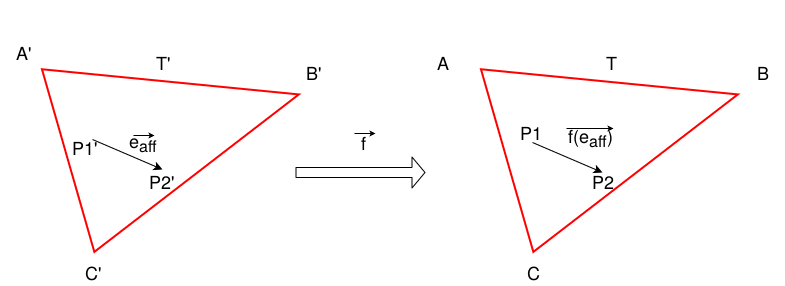
\includegraphics[scale=0.7]{erreur_affine.png}
	\caption{Application affine sur l'erreur de transposition}
	\end{figure}
	En effet à l'intérieur d'un même triangle l'erreur ne dépend pas du point d'application, le vecteur $\overrightarrow{e_{aff}}$ sera donc identique pour chaque point du triangle.

		\subsection{Calcul de l'application affine de l'erreur de transposition}
Afin de pouvoir transposer correctement le point d'intérêt vers l'écran, on doit donc calculer l'application affine normée  $\overrightarrow{f(e_{aff})}$ à partir de ce vecteur $\overrightarrow{e_{aff}}$\\
$$\overrightarrow{e_{aff}} = P2' - P1'$$\\
$$P2'- P1' = f(P2) - f(P1)$$ \\
avec A l'origine du repère \\
$$f(P2) - f(P1) = (A + \overrightarrow{f}(\overrightarrow{AP2})) - (A - \overrightarrow{f}(\overrightarrow{AP1}))$$ \\
$$ = \overrightarrow{f}(\overrightarrow{AP2}) - \overrightarrow{f}(\overrightarrow{AP1}) = 
\overrightarrow{f}(\overrightarrow{AP2} - \overrightarrow{AP1}) = \overrightarrow{f}(\overrightarrow{P1P2})$$ \\
$$= \overrightarrow{f}(\overrightarrow{e_{aff}})$$ \\
Il suffit alors d'étudier l'équation suivante : \\
$$ \overrightarrow{f}(\overrightarrow{e_{aff}}) = \varphi _{2} \times \varphi _{1}^{-1} \times \overrightarrow{e_{aff}}$$ \\
avec les coefficients a,b,c et d calculés auparavant \\
$$ =
		\left(
		\begin{array}{cc}
		a & b \\
		c & d 
		\end{array}
		\right)
		\times
		\left(\begin{array}{c}
		e_{i} \\
		e_{j}
		\end{array}
		\right) =
		\left( 
		\begin{array}{c}
		ae_{i} + be_{j} \\
		ce_{i} + de_{j}
		\end{array}
		\right)
		$$
la norme de $\overrightarrow{f}(\overrightarrow{e_{aff}})$ s'écrit : \\
$$ \parallel \overrightarrow{f}(\overrightarrow{e_{aff}}) \parallel = \sqrt{(ae_{i} + be_{j})^{2}-(ce_{i} + de_{j})^{2}}$$ \\
sachant que \\
$$
\left(
		\begin{array}{cc}
		a & b \\
		c & d 
		\end{array}
		\right)
		\times
		\left(\begin{array}{c}
		e_{i} \\
		e_{j}
		\end{array}
		\right) =
		\left( 
		\begin{array}{c}
		\langle \left(\begin{array}{c}a \\ b \end{array} \right) \mid e \rangle		 \\
		\langle \left(\begin{array}{c}c \\ d \end{array} \right) \mid e \rangle	
		\end{array}
		\right)
		$$ \\
alors \\
$$ \parallel \overrightarrow{f}(\overrightarrow{e_{aff}}) \parallel ^{2} = \langle \left(\begin{array}{c}a \\ b \end{array} \right) \mid e \rangle ^{2} + \langle \left(\begin{array}{c}c \\ d \end{array} \right) \mid e \rangle ^{2} $$ \\
On peut en déduire que \\
$$ \parallel \overrightarrow{f}(\overrightarrow{e_{aff}}) \parallel ^{2} \le ( \parallel \left(\begin{array}{c}a \\ b \end{array} \right) \parallel \cdot \parallel e \parallel) ^{2} + ( \parallel \left(\begin{array}{c}c \\ d \end{array} \right) \parallel \cdot \parallel e \parallel) ^{2}$$ \\
$$ \le \parallel e \parallel ^{2} \cdot( \parallel \left(\begin{array}{c}a \\ b \end{array} \right) \parallel ) ^{2} + ( \parallel \left(\begin{array}{c}c \\ d \end{array} \right) \parallel) ^{2}$$ \\
$$ \parallel \overrightarrow{f}(\overrightarrow{e_{aff}}) \parallel \le \sqrt{\parallel e \parallel ^{2} \cdot( \parallel \left(\begin{array}{c}a \\ b \end{array} \right) \parallel ) ^{2} + ( \parallel \left(\begin{array}{c}c \\ d \end{array} \right) \parallel) ^{2}}$$
Conclusion \\
Avec a,b,c et d à leurs valeurs maximales la norme de $\overrightarrow{f}(\overrightarrow{e_{aff}})$ est \\
$$ \parallel \overrightarrow{f}(\overrightarrow{e_{aff}}) \parallel ^{2} \le \parallel e \parallel \cdot \sqrt{a^{2} + b^{2} + c^{2} + d^{2}} $$ \\
Tous les triangles issus de la calibration sont égaux, ainsi l'erreur sera bornée par les mêmes coefficients a,b,c et d. Afin de travailler dans le cas où l'erreur $\overrightarrow{f}(\overrightarrow{e_{aff}})$ est égale à sa valeur la plus élevée, on fixe les coefficients a,b,c et d à leurs valeurs maximales. \\
Une fois l'erreur de transposition fixée, elle s'ajoutera aux autres erreurs accumulées afin de valider l'algorithme ou bien de procéder au dimensionnement du matériel.

		\subsection{Cas particulier}
Lors de la transposition il est possible que le vecteur $\overrightarrow{e_{aff}}$ correspondant à l'erreur de transposition envoie le point transposé dans un autre triangle que celui où il se trouve initialement. Le cas est représenté à la figure 2.3. Afin de calculé l'erreur via la méthode présentée précédemment, on identifie deux vecteurs $\overrightarrow{f1}$ et $\overrightarrow{f2}$ dont la somme est égale au vecteur $\overrightarrow{e_{aff}}$. Chacun de ces vecteurs devant se situer respectivement dans un triangle indépendant concerné par le chevauchement\\
Dans l'exemple représenté dans la figure 2.3, $\overrightarrow{f1}$ appartient au triangle T1 et $\overrightarrow{f2}$ appartient au triangle T2.
$$\parallel \overrightarrow{e_{aff}} \parallel \le \parallel \overrightarrow{f1} \parallel + \parallel \overrightarrow{f2} \parallel $$ \\
$$ \le \parallel \overrightarrow{f1} \parallel \cdot \sqrt{a^{2} + b^{2} + c^{2} + d^{2}} + \parallel \overrightarrow{f2} \parallel \cdot \sqrt{a^{2} + b^{2} + c^{2} + d^{2}}$$
\begin{figure}[!h]
	\centering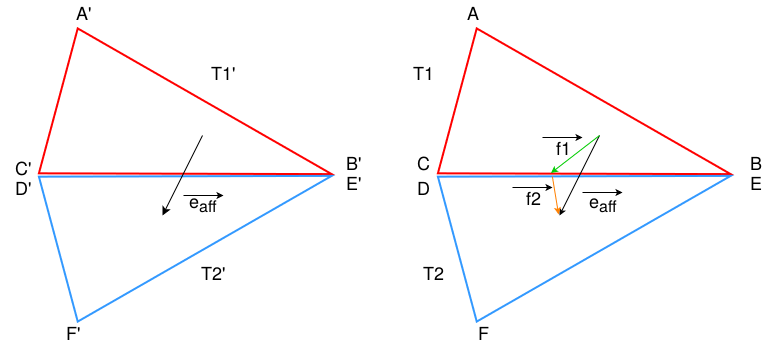
\includegraphics[scale=0.7]{erreur_affine2.png}
	\caption{Application affine sur l'erreur de transposition lorsque le vecteur $ \overrightarrow{e _{aff}}$ chevauche deux triangles }
\end{figure}

\newpage

        \section{Détection du cadre de référence}
        	\subsection{Principe}
            Afin d'affirmer que la création du cadre de référence est correcte et que la détection des lunettes par un algorithme est suffisamment précise, nous devons tester celui-ci. Une collection d'images est créée grâce à un protocole expérimental précis et reproductible. Lors de ce protocole plusieurs positions de caméra autour d'un écran, angles d'inclinaison vers l'avant et vers l'arrière mais aussi des angles de rotation vers la droite et vers la gauche de la caméra sont utilisés. Une tête de mannequin munie des lunettes est positionnée face à l'écran selon différents angles d'inclinaison et de rotation. \\
        Cette collection d'image est traitée par l'algorithme de détection du cadre testé et les coordonnées déterminées par celui-ci sont enregistrées. Un second programme permet d'établir des coordonnées de références de la collection d'images manuellement. Via un évènement click souris effectué par l'utilisateur, des coordonnées de références des cadres sont enregistrées. Enfin, un troisième programme compare les deux jeux de coordonnées et indique la précision de l'algorithme de détection du cadre de référence en prenant en compte l'erreur tag. 
            \subsection{Erreur tag de l'utilisateur}
            La précision de l'utilisateur lors du tag de la collection d'image n'étant pas parfaite, un test est à réaliser pour déterminer la précision du tag manuel. Dans le but de quantifier ce que l'on appellera $eu_{ref}$, l'opération de tag doit être réalisée plusieurs fois sur un lot d'images afin de comparer les coordonnées données pour une même image et en déduire l'erreur de tag. Une moyenne d'erreur sera réalisée sur le jeu d'images utilisé et correspondra à l'erreur de tag nécessaire pour les calculs à venir.
            \subsection{Calcul de l'erreur et interprétation}
        \section{Détection du centre de l'iris}
        	\subsection{Principe}
             Un test de l'algorithme de détection prouvant que celui-ci permet effectivement de donner une position correcte du centre de l'iris dans un cadre de référence est indispensable à la validation de notre modèle. L'utilisation d'un tel algorithme implique la présence d'une erreur dite "réelle" qui existe entre la vraie position du centre de l'iris et la position détectée par l'algorithme. Le but lors de cette étape est de quantifier cette erreur afin de pouvoir la prendre en compte lors de l'affichage du curseur à l'écran.\\
    A l'instar de la détection du cadre de référence, une collection d'images est créée, en amont du test, grâce à un protocole expérimental précis et reproductible. Ce protocole permet de reproduire les positions potentielles de l'iris dans l'espace. La position de la caméra, l'angle d'inclinaison et l'angle de rotation s'ajouteront à 9 points de repères affichés à l'écran que l'utilisateur devra fixer successivement afin de composer une collection d'images suffisamment dense et diversifiée. \\
    Le test se déroule en trois étapes :
    
\begin{itemize}
\item Un programme prend en entrée la collection d'images créée, soumet ces images à l'algorithme de détection de l'iris qui renvoie les coordonnées du centre de l'iris de chaque oeil. Ces coordonnées sont ensuite stockées dans un fichier texte indépendant.
\item Un second programme utilise également la collection d'images. Ici l'utilisateur doit positionner manuellement le centre de l'iris de chaque oeil sur chaque image de la collection. Cette opération est appelée "tag de l'iris". Chacune des coordonnées obtenues ici est stockée dans un fichier texte selon la même logique que pour l'algorithme de détection.
\item La dernière partie de ce test correspond à l'étape de comparaison des jeux de coordonnées stockées lors des étapes précédentes. Cette opération permet l'interprétation des résultats, c'est à dire de pouvoir quantifier l'erreur réelle liée à l'algorithme utilisé et tout simplement d'affirmer ou d'infirmer le bon fonctionnement de cet algorithme.
\end{itemize}

\subsection{Algorithme de détection de l'iris}
Comme énoncé précédemment le premier programme utilisé lors de ce test permet de déterminé pour chaque image et pour chaque oeil la position du centre de l'iris détectée par l'algorithme de détection testé. Pour rappel, la détection de l'iris est réalisée dans le cadre de référence dessiné au préalable sur l'image, les coordonnées correspondent donc à la position de l'iris dans ce cadre de référence. On notera donc le centre de l'iris détecté par l'algorithme pour un oeil.

\subsection{Tag manuel de l'iris}
Ce programme permet donc à l'utilisateur de déterminer manuellement la position du centre de l'iris de chaque oeil dans chaque image issue de la collection. Afin de pouvoir comparer les coordonnées obtenues ici avec celles obtenues via l'algorithme de détection ce tag sera réalisé dans le cadre de référence dessiné auparavant. \\ 
Cette étape de tag devant être à la fois précise et fiable, une contrainte liée à ce tag doit être mise en place. Un cercle de rayon rt et de centre t est tracé à l'écran, l'utilisateur doit placer le point t sur le centre de l'iris et le cercle doit être strictement inclus dans l'iris afin que le tag soit validé. Si l'utilisateur ne peut pas placer le cercle entièrement dans l'iris, le tag est dit invalide et l'image est rejetée par l'utilisateur.\\ 
On considère dans ce modèle que la pupille ainsi que l'iris de l'oeil sont deux cercles parfaits en deux dimensions. On défini donc r comme le rayon de l'iris, r prendra une valeur fixe pour chaque utilisateur et ce tout au long de l'utilisation du programme. Pour respecter nos calculs, nous considérons que la taille de l'iris de l'utilisateur est constante pour l'ensemble de la collection d'image et donc que r est fixe pour chaque utilisateur. \\
r sera déterminé manuellement lors d'une étape de pré-mesure par l'utilisateur au lancement du test complet. Le calcul de rt (rayon du cercle autour du tag) sera conditionné par le fait que $r<rt$, dans le cas contraire l'opération de tag sera impossible.\\
Le calcul du rayon rt est effectué avant l'étape de tag, cette valeur est obtenue grâce à l'équation suivante : \\
$$rt = r - e_{aff} + 1 - eu_{iris}$$ \\
avec $e_{aff}$ l'erreur issue de l'algorithme barycentrique et eu l'erreur liée au facteur humain lors de l'étape de tag. On ajoute 1 pixel lors de l'opération afin que rt ne soit pas exactement égal à la somme des erreurs permises.\\ L'erreur eu est calculée grâce à un autre test indépendant. Un jeu d'images issue de la collection réalisée en amont sert de support pour ce test. Il s'agit pour l'utilisateur de tagger à plusieurs reprises un lot répété d'images et de comparer les coordonnées obtenues afin d'en déduire une erreur de manipulation, appelée $eu_{iris}$ ici. \\
Suite au calcul de rt, on est capable de définir une zone zt qui correspond à l'ensemble des positions potentielles de t; zt est un cercle de rayon r-rt.

\subsection{Calcul de l'erreur réelle et interprétation}
Une fois les valeurs de r et rt fixées ainsi que les points t et d positionnés sur l'image, l'enjeu est de quantifier l'erreur existante entre la véritable position du centre de l'iris et la position détectée par l'algorithme, on note cette erreur $e_{iris}$. On veut borner cette erreur de manière à qu'elle soit négligeable, elle doit donc avoir une valeur la plus petite possible. On défini c comme le vrai centre de l'iris. Ne connaissant pas la position réelle de c mais connaissant la position de d et t tout deux ne représentant pas la réalité, nous pouvons en déduire une valeur qui sera supérieure ou égale à la distance entre c et d, en d'autres mots l'erreur $e_{iris}$ sera inférieure ou égale à cette valeur déduite.\\ 
On considère l'erreur mesurée, notée $e_{m}$, correspondant à la distance en pixel entre le point d et t.\\ 
Il existe une relation entre les points d, t et c telle que : \\
$$cd < ct + td $$\\
De plus on sait que t est inclus dans la zone zt (cercle de rayon r-rt)\\
$$cd < r - rt + e_{m}$$ \\
$e _{iris}$ correspondant à la distance entre c et d,\\
$$e_{iris} < r - rt + e_{m}$$ \\
Dans le cas où d, t et c sont alignés,\\
$$cd = ct + td$$ \\
alors l'erreur réelle est exactement égale à la somme des distances ct et td\\
$$e_{iris} = r - rt + e_{m}$$ \\
de plus on sait que la somme des distances ct et td doit être inférieure à l'erreur permise $e_{3}$ issue de la différence entre l'erreur maximale et l'erreur $e_{aff}$ définies au préalable, on obtient alors : \\ 
$$e_{iris} \leq e_{3} $$ \\
Notre erreur réelle $e_{iris}$ est alors bornée par cette valeur $e_{3}$, ce qui nous permet de déduire si la résolution de l'image utilisée est suffisante ou non pour répondre aux exigences liées aux erreurs des différents algorithmes utilisés dans ce logiciel. 


    \begin{figure}
    \centering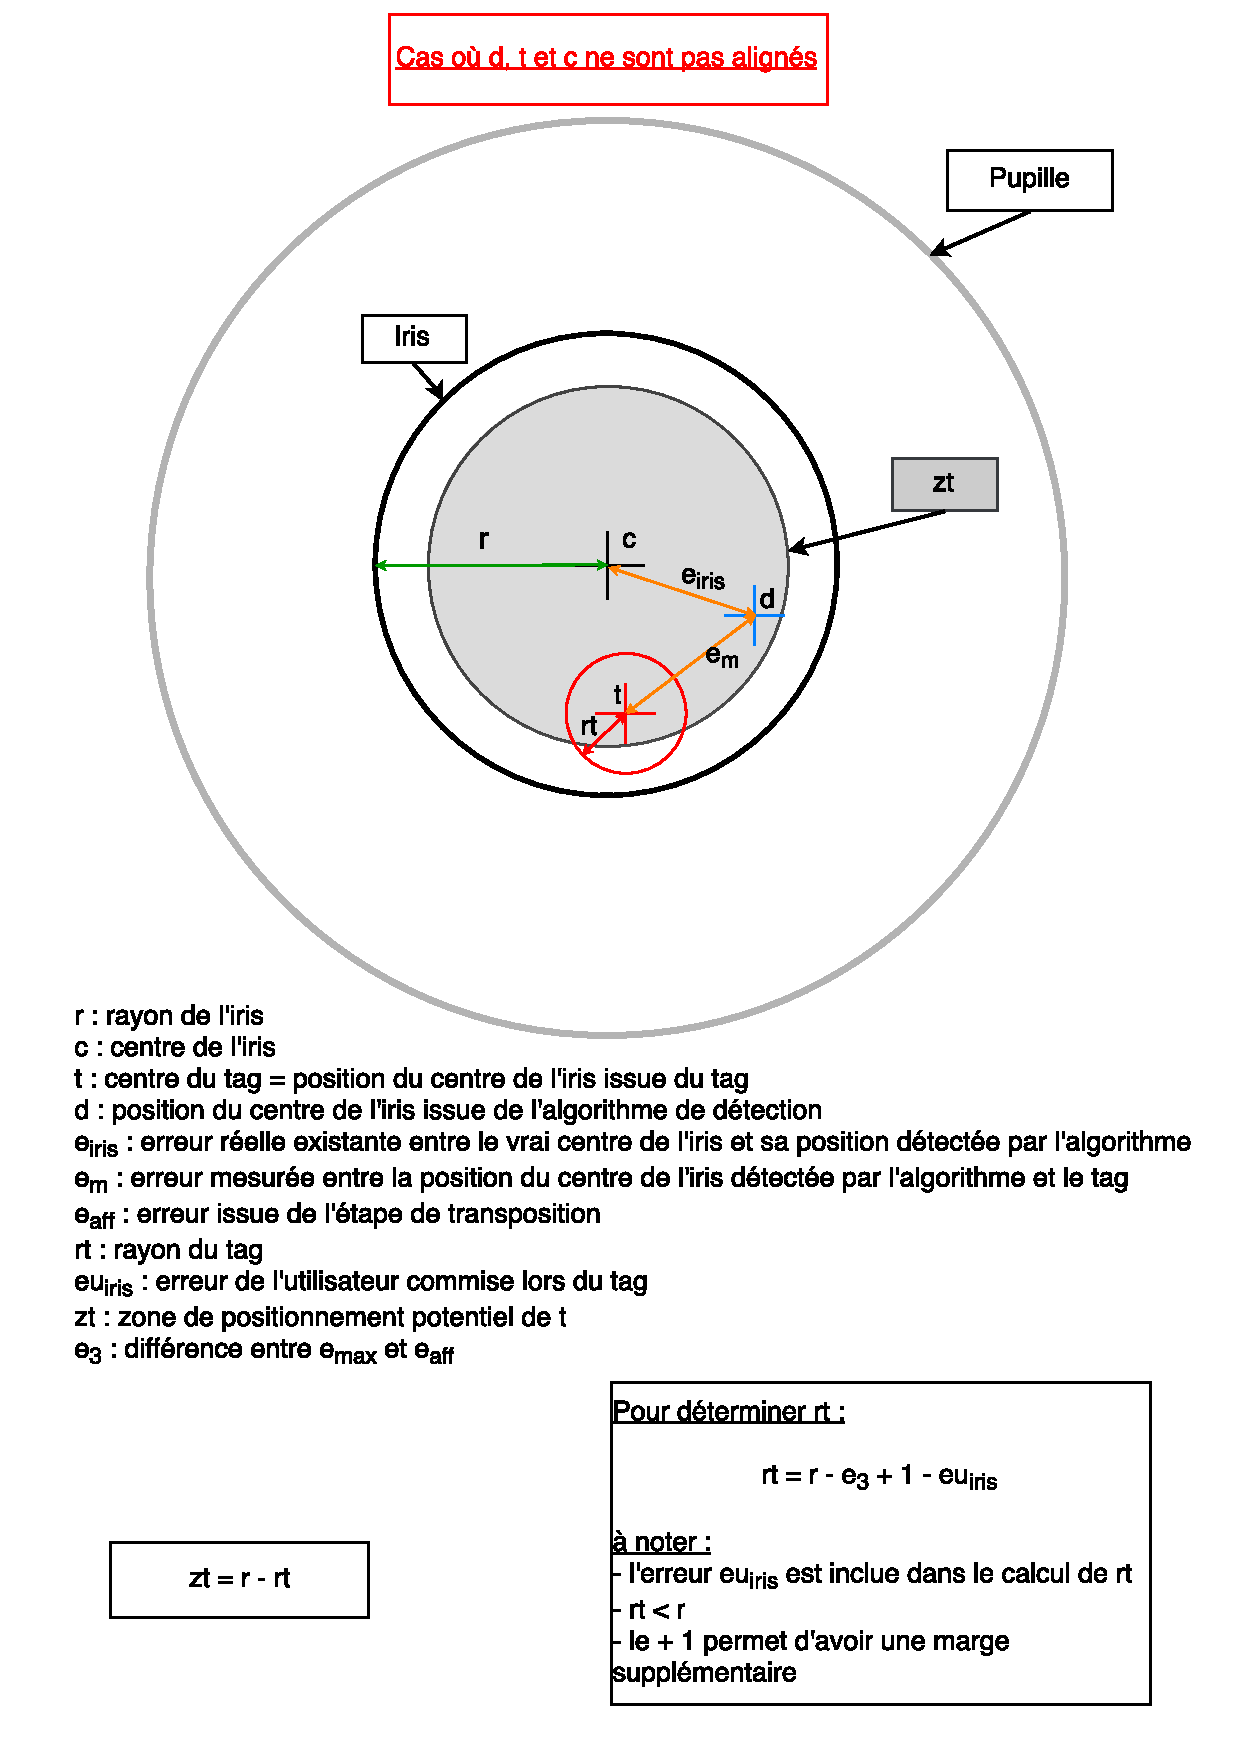
\includegraphics[height=24cm]{erreur_oeil_1.pdf}
    \end{figure}
    \begin{figure}
    \centering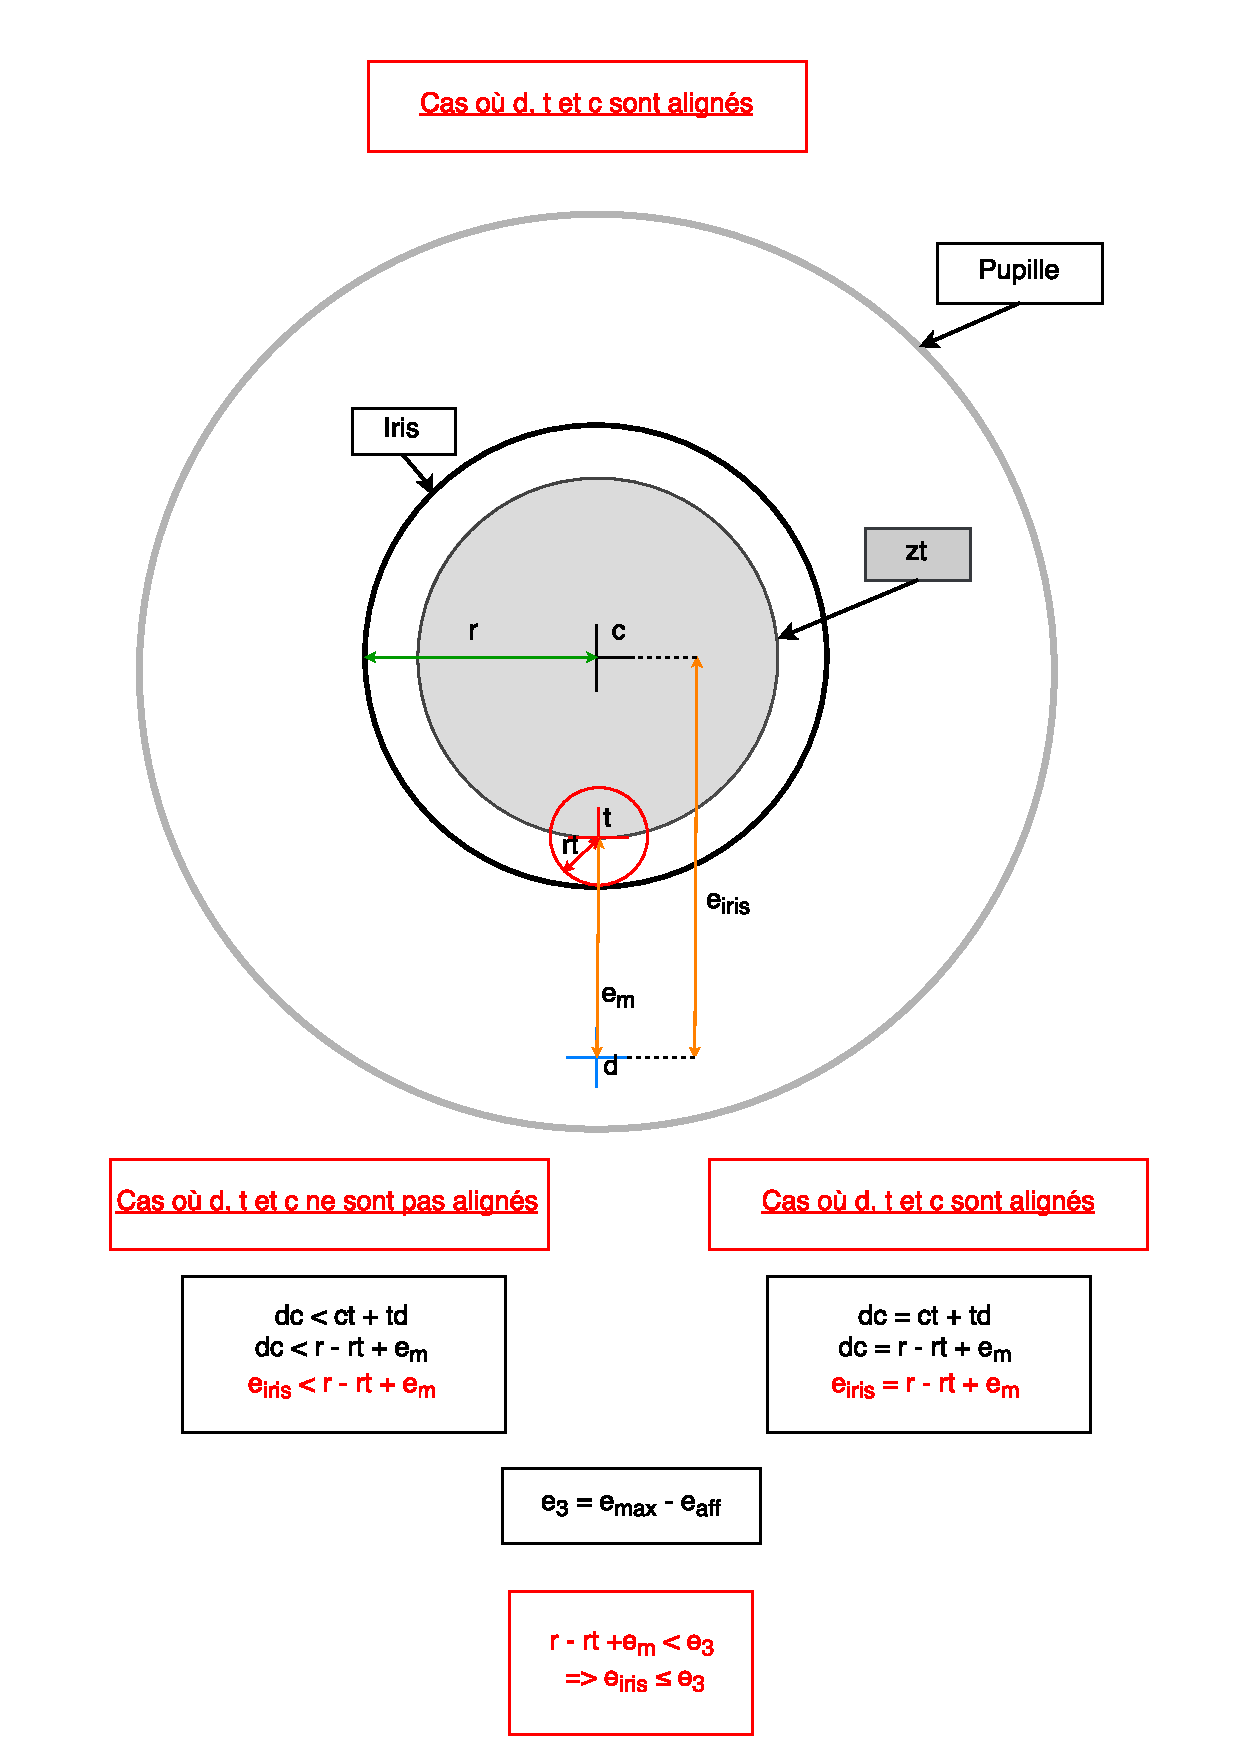
\includegraphics[height=24cm]{erreur_oeil_2.pdf}
	\caption{Schéma détermination de l'erreur $e_{iris}$ générée par l'algorithme de détection de l'iris}
	\end{figure}
    \newpage

    \section{Gui (Graphic user interface)}
Au cours de l'utilisation du logiciel, quatre fenêtres seront affichées à l'écran afin de pouvoir contrôler le placement des différents cadres de références et des centres de l'iris détectés en temps réel. La vidéo brute, l'affichage des cadres de références ainsi que la détection de l'iris pour chaque oeil seront ainsi visibles par l'utilisateur.
    \begin{figure}[h]
    \centering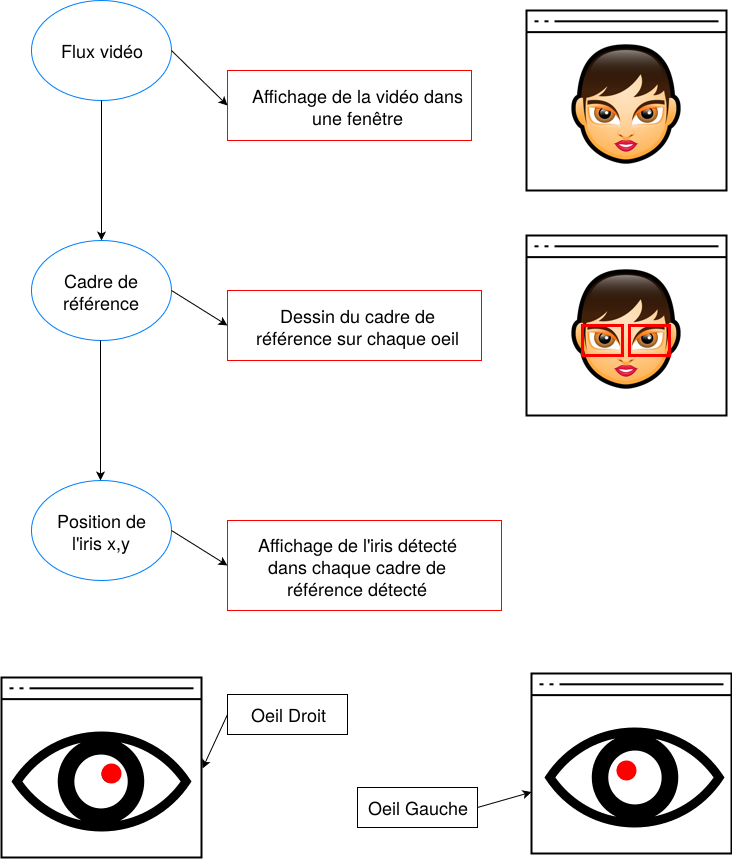
\includegraphics[height=18cm]{gui.png}
    \caption{Schéma du GUI sur la détection du cadre de référence et du centre de l'iris}
    \end{figure}
    \newpage
	\chapter*{Flux de tâches pour la validation du modèle}
	La figure 2.5 ci-dessous récapitule les tests à effectuer pour le calcul des erreurs générés par les algorithmes.
    \begin{figure}[!h]
    \centering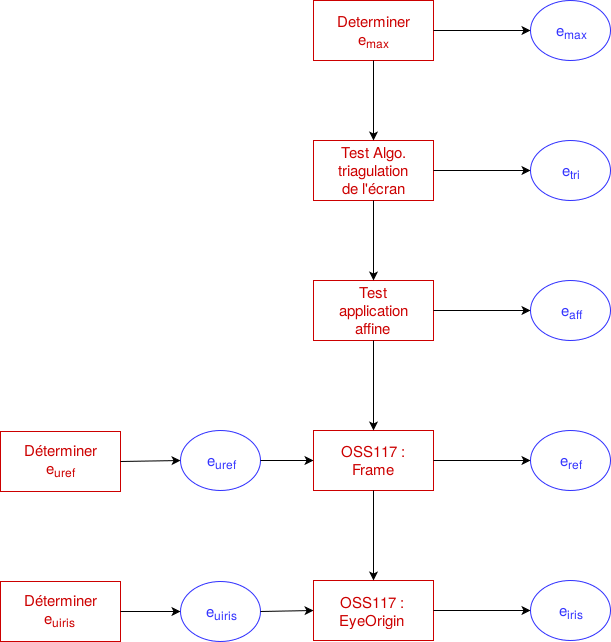
\includegraphics[height=15cm]{Workflowtest.png}
    \caption{Flux des tests}
    \end{figure}
    \newpage
\begin{thebibliography}{}
\addcontentsline{toc}{chapter}{References}
\bibitem{c1}OpenCV (Open Computer Vision) est une bibliothèque graphique libre spécialisée dans le traitement d'images en temps réel. www.opencv.org
\bibitem{c2}Applications affines, Cours, M@ths en lIgne, Université de Grenoble 2011
\end{thebibliography}{}

\end{document}

%Redigé par  Théo Falgarone et Tristan Maunier 